\documentclass{article}
\usepackage[utf8]{inputenc}
\usepackage[spanish]{babel}
\usepackage{listings}
\usepackage{graphicx}
\graphicspath{ {images/} }
\usepackage{cite}

\begin{document}

\begin{titlepage}
    \begin{center}
        \vspace*{1cm}
            
        \Huge
        \textbf{Informe}
            
        \vspace{0.5cm}
        \LARGE
        Parcial 1
            
        \vspace{1.5cm}
            
        \textbf{Juan Camilo Mazo Castro}
            
        \vfill
            
        \vspace{0.8cm}
            
        \Large
        Despartamento de Ingeniería Electrónica y Telecomunicaciones\\
        Universidad de Antioquia\\
        Medellín\\
        Abril de 2021
            
    \end{center}
\end{titlepage}

\tableofcontents
\newpage
\section{Analisis del problema}\label{intro}
Informa2 S.A.S. solicita una matriz de leds para mostrar mensajes o patrones en la fachada de su negocio. Se requiere que el dispositivo cuente con 3 opciones las cuales son:\\\\
1.	Verificar que los 64 leds se encuentran en buen estado y que pueden encenderse.\\
2.	Mostrar en pantalla una imagen o patrón de forma fija.\\
3.	Mostrar en pantalla varias imágenes o patrones de forma secuencial. También debe permitir escoger el número de patrones que se van a mostrar.\\\\
Lo primero para la solución del problema es crear un circuito que haga una conexión entre el monitor serial y la matriz de leds. Seguido de lo anterior se procede a la creación del algoritmo que hace posible la interacción entre los valores que ingrese el usuario por el monitor serial y la matriz de leds para ejecutar las diferentes funcionalidades del dispositivo.\\\\

\section{Consideraciones} \label{consideraciones}
Lo primero que se tuvo en cuenta fue la cantidad de Arduinos disponibles, ya que solo se contaba con uno y este solo tenía disponibles siete de sus puertos. Por otro lado, se contaba con varios 74HC595 que fueron muy bien aprovechados para poder lograr el objetivo y solucionar la falta de Arduino y puertos. Se utilizaron tres de los puertos del Arduino y estos se conectaron a ocho 74HC595 conectados secuencialmente con ayuda del pin nueve de los chips. Seguido de lo anterior, se asignaron ocho leds a cada uno de los 74HC595 y se hicieron las respectivas conexiones con resistencias.\\
Finalizada la etapa de la creación del circuito, se empezó a implementar el algoritmo para el dispositivo. Este se basa en la creación de una matriz de 8x8 posiciones, la cual le asignara cada una de sus posiciones a uno de los leds. El algoritmo le pide al usuario números entre el uno y el ocho que son respectivamente los puestos de los leds en cada una de las columnas (Figura1), es decir que el usuario debe indicar qué leds en cada una de las columnas desea que sean encendidos. Una vez el usuario ingresa los números de las columnas se sigue el esquema de la (Figura2). Por otro lado, para la “verificación” se realiza encendiendo todos los leds mediante el envío del numero binario 11111111 ocho veces por el serial al 74HC595.

\begin{figure}[h]
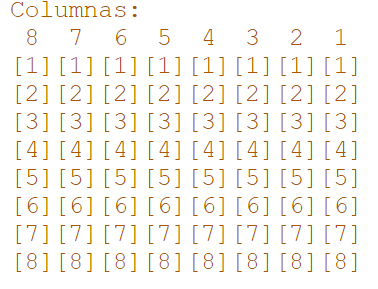
\includegraphics[width=8cm]{Figura1.png}
\centering
\caption{Matriz de 8x8.}
\label{fig:Matriz}
\end{figure}

\begin{figure}[h]
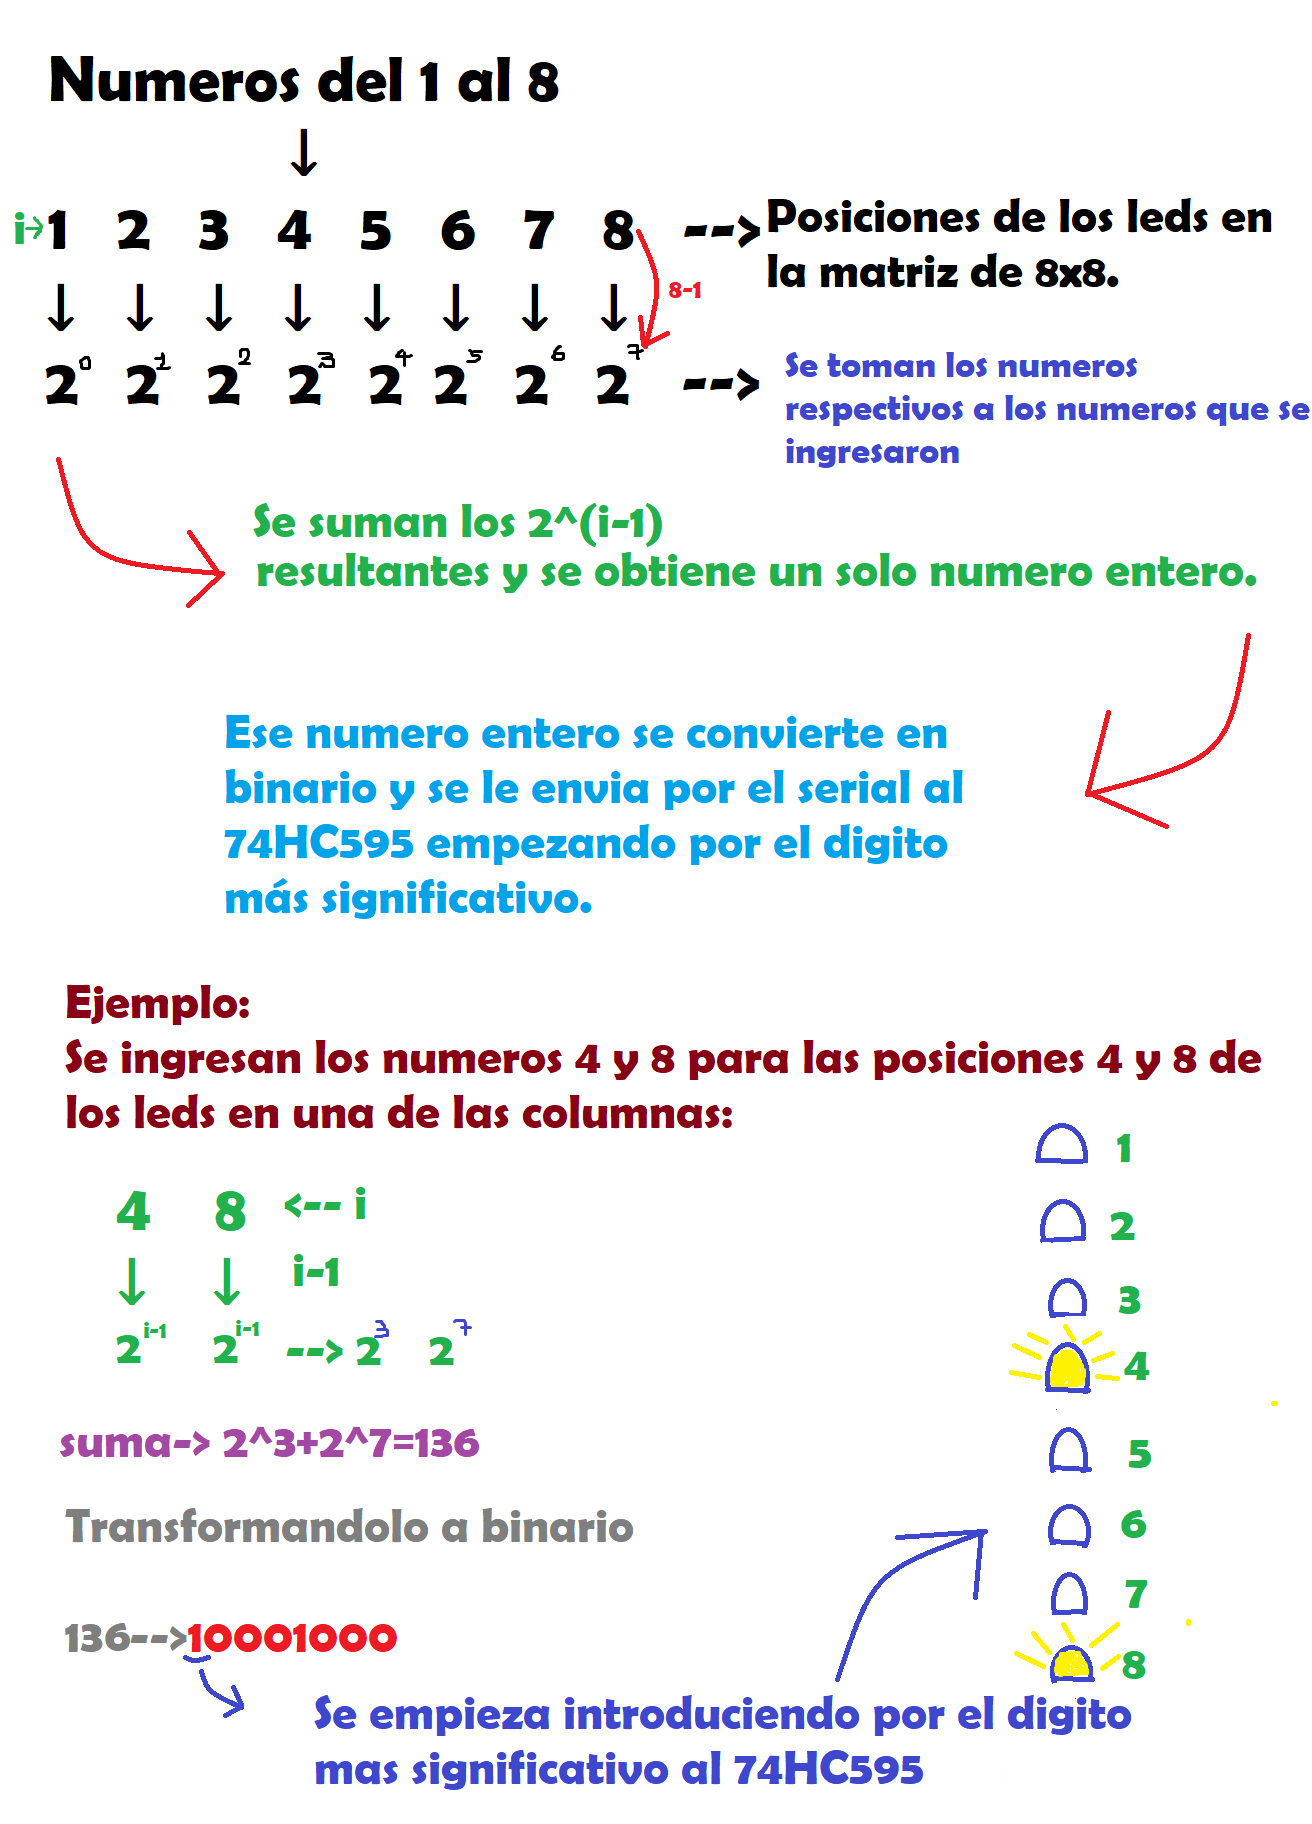
\includegraphics[width=8cm]{Figura2.png}
\centering
\caption{Esquema algoritmo}
\label{fig:Esquema}
\end{figure}

\section{Tareas realizadas} \label{tareas}
Las tareas realizadas para el desarrollo del proceso en la (Figura2) fueron las siguientes:\\\\
1. Realizar un menú para verificar qué se desea hacer.\\
2. Si se desea hacer la verificación, encender todos los leds de la manera antes dicha.\\
3. Si por otro lado desea usar imagen o publik, se empiezan a solicitar números del 1 al 8 para llenar las columnas.\\ 
4. Se utiliza un ciclo para sumar los números 2 que se encuentran elevados a cada uno de los números ingresados menos 1.\\
5. En el proceso anterior se obtiene un numero decimal que en binario representa el numero que debe ser enviado al 74HC595 para que encienda los leds en las posiciones respectivas a los números que se ingresaron.\\
6. Se convierte el numero decimal a binario y a este se le envían cada uno de sus dígitos de izquierda a derecha por medio de los puertos del Arduino.\\
7. En la función imagen el anterior proceso se repite 8 veces, el 74HC595 empieza encendiendo los leds de la columna número 8 de la (Figura1), Al seguir ingresando los binarios, los leds encendidos se irán corriendo a la columna siguiente hacia la derecha.\\
8. Para la función publik, se sigue el mismo proceso que con imagen, pero se repite el proceso de llenar toda la matriz un número de veces igual al número de patrones que se desea que se impriman.\\\\

\section{Problemas presentados durante el desarrollo} \label{problems}
Los mayores problemas que se presentaron durante el desarrollo del parcial estuvieron relacionados con Tinkercad y las diferentes fallas que esta plataforma presentaba. En el momento en que se ponen una buena cantidad de dispositivos en el circuito Tinkercad se vuelve bastante lento, por lo que se dificulta el uso de la mismo.\\
En uno de los intentos de armar el circuito sucedió que no se podían borrar unos elementos que estaban mal puestos, se intentó darles borrar pero estos no desaparecían, incluso refrescando la página o cerrando y abriendo nuevamente la página se seguía presentando nuevamente el problema, por lo que se tuvo que iniciar nuevamente toda la construcción en un nuevo circuito.\\
En el segundo intento para armar el circuito sucedió en un par de ocasiones que se perdía la conexión con el servidor sin que se perdiera el internet del computador. A pesar de lo anterior se logró terminar el circuito y cuando se empezó a escribir el código del programa, por un momento sucedió que no se podía escribir absolutamente nada porque se borraba inmediatamente, es decir que no podía escribir nada nuevo. La solución para el problema anterior fue crear una duplicación del circuito, luego de esto se realizaron varias copias de seguridad para posibles fallas ya que se pudo observar que la plataforma no era muy estable.\\
Finalmente, el último inconveniente que hubo fue a la hora de pasar el código que se tenía en Qt para Tinkercad, ya que al pasarlo había que cambiar los “cin” y los “cout” por las respectivas instrucciones del serial en Tinkercad. Al principio no se obtenían los resultados esperados por un mal manejo del serial, y se tuvo que hacer uso del debugger de la plataforma para encontrar el error, dicho debugger funcionaba muy mal, pues indicaba que se encontraba la ejecución en uno de los breakpoints que se ponían, pero a la vez el monitor serial se quedaba pegado imprimiendo a medias un print que se encontraba más arriba que el breakpoint, por lo que no parece que el debug funcione sincronizado con la ejecución.\\\\


\section{Evolución algoritmo} \label{evolucion}
de que el usuario pudiera seleccionar los leds en cada una de las columnas para así enseñar cualquier patrón que se desee.\\
Se sabía que se necesitaba un numero binario de 8 bits para prender cada una de las columnas de la matriz de leds, pero para no hacer que el usuario ingresara unos y ceros, se realizaron las funciones para que el usuario ingrese números del 1 al 8, así producir un dispositivo más sencillo de usar para el usuario. Fue así como se observó que los números del 1 al 8 en cada uno de las columnas podía ser representados como un numero decimal que convertido a binario tiene los dígitos que deben ser ingresados al 74HC595 para que prenda los leds de las respectivas posiciones que el usuario requiere. 


\end{document}
